% Drawing 154/08-24 -- folder 154, batch 08, archive page 154 (PDF page 155).
% Transcription: trois dessins, marqués au crayon $(\mathrm{I}_1)$, $(\mathrm{I}_2)$, $(\mathrm{I}_3)$ : une droite verte horizontale (la position de départ), bordée de deux courbes brunes numérotées $1$ (au-dessous) et $2$ (au-dessus), entre deux traits verticaux en tirets ; au crayon, des faisceaux de droites de $\Sigma$ passant par des sommets marqués. Dans $(\mathrm{I}_1)$, la courbe $2$ fait une bosse en tirets pour passer par le sommet $a$ ; dans $(\mathrm{I}_2)$, les deux courbes s'écartent en un fuseau, $2$ passant par $a$ en haut et $1$ par $b$ en bas, une flèche double brune de $b$ à $a$ ; dans $(\mathrm{I}_3)$, $2$ passe par $a$ et $b$, $1$ par $c$, un chemin de flèches brunes $a$, $c$, $b$. Au-dessous, le dessin $(\mathrm{I}_n)$ : la même bande, les deux courbes brunes passant alternativement par sept sommets, quatre en haut et trois en bas, reliés par des faisceaux de droites au crayon qui dessinent des zigzags
% Kind: elementary sweeps (I1), (I2), (I3), (In). Method 2 (schematic redraw from the facsimile). Status: partial.
% Notes: Four drawings; the braces and the texts under them belong to the text. (I_1): the green line between two vertical dashed strokes, the brown curve 1 just below it, the curve 2 just above it rising in a dashed bump through the vertex a. (I_2): the two brown curves opening into a spindle, 2 through a at the top, 1 through b at the bottom, the brown double arrow from b to a. (I_3): a wider spindle, 2 through a and b, 1 through c, the arrows a to c and c to b. (I_n): a long spindle, four vertices on the upper curve and three on the lower one, the pencil zigzag joining them in turn, the label (I_n) and « (n = 7) ». The pencil sheaves of lines of Sigma through each vertex are left out, as are the three very pale strip sketches at the top of the page (no label, barely visible). The count of seven vertices in (I_n) agrees with the « (n = 7) » written beside it, which settles the transcription's doubt. Redrawn 2026-11-12 (issue 128): to check again. 2026-11-14, Claude Opus 5.5, overlay check (issue 147): rasterised from its own coordinates over the 400 dpi colour scan (402 ppi native) on a unit grid; not compiled (no TeX in the session). The four bands with their green lines, brown curves, dashed strokes, vertices, brown arrows, labels and the pencil zigzag of (I_n) lie on their ink to within about 1 unit; the redraw is unchanged. Still partial: the pencil sheaves of lines of Sigma through the vertices, which the transcription names (four to six faint lines through each of the thirteen vertices), are not drawn, nor are the three pale strip sketches at the top of the page.
% Coordinates: 1 unit = 1 mm = 1/100 of the crop width (bbox in page fractions: [0.105, 0.085, 0.985, 0.535]).
% Redrawn by Claude (claude-fable-5-2), issue #128, 2026-11-12; not checked by a human; not compiled (no TeX in the session).
% Checked by Claude (claude-opus-5-5) 2026-11-14 (issue #147): overlaid on the 400 dpi colour facsimile; not compiled (no TeX in the session). Not checked by a human. Status: partial.
% Rights: reproduces part of the work -- behind RENDER_TRANSCRIPTS, never published by itself.
\documentclass[tikz,border=3pt]{standalone}
\usepackage{amsmath,amssymb}
\usetikzlibrary{patterns,arrows.meta}
\tikzset{Dg/.style={green!45!black}, Br/.style={brown!80!black}, pencil/.style={black!45}, struck/.style={black!35}, mpt/.style={circle,draw,inner sep=1.3pt}, pt/.style={circle,fill,inner sep=0.9pt}, opt/.style={circle,draw,fill=white,inner sep=1.1pt}}
\begin{document}
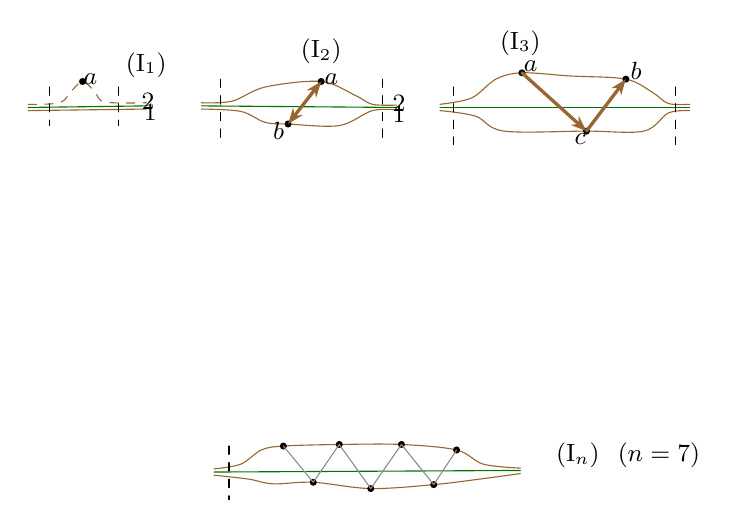
\begin{tikzpicture}[x=1mm,y=1mm,line cap=round,line join=round,font=\scriptsize]
\node[inner sep=1pt] at (23.4,-15.7) {\small $(\mathrm{I}_1)$};
\draw[Dg] (8.4,-21.1) -- (23.4,-20.9);
\draw[Br] (8.4,-21.5) -- (23.4,-21.3);
\draw[Br,dashed] plot[smooth, tension=0.55] coordinates {(8.4,-20.7) (12.4,-20.5) (13.9,-19) (15.3,-17.8) (16.8,-19) (18.1,-20.4) (23.4,-20.5)};
\draw[dashed] (11.1,-18.5) -- (11.1,-23.4);
\draw[dashed] (19.9,-18.5) -- (19.9,-23.4);
\node[pt] at (15.3,-17.8) {};
\node[inner sep=1pt] at (16.3,-17.5) {\small $a$};
\node[inner sep=1pt] at (23.6,-20.3) {\small 2};
\node[inner sep=1pt] at (23.9,-21.8) {\small 1};
\node[inner sep=1pt] at (45.6,-14) {\small $(\mathrm{I}_2)$};
\draw[Dg] (30.4,-20.9) -- (55.2,-21.1);
\draw[Br] plot[smooth, tension=0.55] coordinates {(30.4,-20.5) (34.3,-20.3) (38.5,-18.5) (45.6,-17.8) (50,-19.6) (52.1,-20.7) (55.2,-20.8)};
\draw[Br] plot[smooth, tension=0.55] coordinates {(30.4,-21.3) (35.4,-21.6) (38.5,-23) (41.4,-23.2) (47.9,-23.4) (52.1,-21.5) (55.2,-21.4)};
\draw[dashed] (32.8,-17.5) -- (32.8,-25.3);
\draw[dashed] (53.4,-17.5) -- (53.4,-25.3);
\node[pt] at (45.6,-17.8) {};
\node[pt] at (41.4,-23.2) {};
\draw[Br,very thick,{Stealth[length=2mm]}-{Stealth[length=2mm]}] (41.4,-23.2) -- (45.6,-17.8);
\node[inner sep=1pt] at (46.9,-17.5) {\small $a$};
\node[inner sep=1pt] at (40.2,-24.1) {\small $b$};
\node[inner sep=1pt] at (55.5,-20.6) {\small 2};
\node[inner sep=1pt] at (55.5,-22) {\small 1};
\node[inner sep=1pt] at (70.9,-12.9) {\small $(\mathrm{I}_3)$};
\draw[Dg] (60.7,-21.1) -- (92.4,-21.1);
\draw[Br] plot[smooth, tension=0.55] coordinates {(60.7,-20.7) (64.7,-19.9) (67.8,-17.5) (71.1,-16.7) (77.2,-17.1) (84.3,-17.5) (87.7,-19.2) (89.7,-20.6) (92.4,-20.7)};
\draw[Br] plot[smooth, tension=0.55] coordinates {(60.7,-21.5) (65.2,-22.2) (68.8,-24.1) (79.3,-24.1) (86.6,-24.1) (89.7,-21.8) (92.4,-21.5)};
\draw[dashed] (62.4,-18.5) -- (62.4,-25.8);
\draw[dashed] (90.6,-18.5) -- (90.6,-25.8);
\node[pt] at (71.1,-16.7) {};
\node[pt] at (84.3,-17.5) {};
\node[pt] at (79.3,-24.1) {};
\draw[Br,very thick,-{Stealth[length=2mm]}] (71.1,-16.7) -- (79.3,-24.1);
\draw[Br,very thick,-{Stealth[length=2mm]}] (79.3,-24.1) -- (84.3,-17.5);
\node[inner sep=1pt] at (72.2,-15.9) {\small $a$};
\node[inner sep=1pt] at (85.6,-16.5) {\small $b$};
\node[inner sep=1pt] at (78.5,-25.1) {\small $c$};
\draw[Dg] (32,-67.4) -- (70.9,-67.2);
\draw[Br] plot[smooth, tension=0.55] coordinates {(32,-67) (35.4,-66.4) (38,-64.6) (40.8,-64.1) (47.9,-63.9) (55.8,-63.9) (62.8,-64.6) (66.2,-66.4) (70.9,-66.9)};
\draw[Br] plot[smooth, tension=0.55] coordinates {(32,-67.8) (36.4,-68.3) (39.5,-68.9) (44.6,-68.7) (51.9,-69.5) (59.9,-69) (65.7,-68.3) (70.9,-67.6)};
\draw[dashed] (33.9,-64.1) -- (33.9,-70.9);
\node[pt] at (40.8,-64.1) {};
\node[pt] at (47.9,-63.9) {};
\node[pt] at (55.8,-63.9) {};
\node[pt] at (62.8,-64.6) {};
\node[pt] at (44.6,-68.7) {};
\node[pt] at (51.9,-69.5) {};
\node[pt] at (59.9,-69) {};
\draw[pencil] (40.8,-64.1) -- (44.6,-68.7) -- (47.9,-63.9) -- (51.9,-69.5) -- (55.8,-63.9) -- (59.9,-69) -- (62.8,-64.6);
\node[inner sep=1pt] at (78.2,-65.3) {\small $(\mathrm{I}_n)$};
\node[inner sep=1pt] at (88.5,-65.3) {\small $(n=7)$};
\end{tikzpicture}
\end{document}
